\subsection{Описать явление «холодной» эмиссии. Рассматривая металл как потенциальный ящик
конечной глубины заполненный «свободными» электронами, получить зависимость для плотности
тока $J$ «холодной» эмиссии от напряженности приложенного поля. Объяснить, почему холодная
эмиссия не может быть объяснена классической физикой}

Холодная эмиссия -- излучение/испускание электронов из твердого тела за счет туннельного
эффекта. Аналогично термоэлектронной эмиссии, есть катод, с которого будут вылетать электроны,
он погружён в вакуум, над поверхностью катода пластина -- анод, которая ловит электроны и мы 
смотрим ток, создаваемый ими. (см. устную часть, 2.4.4 -- ТЭЭ во внешнем электрическом поле).
Потенциальная энергия в зависимости от $x$ -- расстояния от поверхности металла: 
$U(x) = U_0 - e \varepsilon x, x>0$.
\begin{figure}[H]
  \centering
  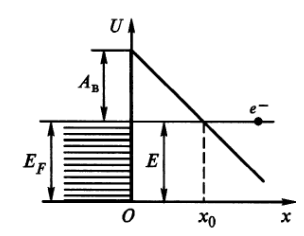
\includegraphics[width=.9\linewidth]{img/write-08/barier.png}
  \caption{Вид потенциала при холодной эмиссии}
  \label{fig:cold-emission}
\end{figure}

Вероятность туннелирования электрона определяется
коэффициентом прохождения $D$ через потенциальный барьер:
\[
  J_{\varepsilon} \sim D = exp \left\{ - \dfrac{2}{\hbar} \int_0^{x_0} \sqrt{2m_e (U(x) - E)} \, dx \right\},
\]
где $x_0$ удовлетворяет уравнению
$U(x_0) = E_F \Leftrightarrow x_0 = \dfrac{U_0 - E_F}{e \varepsilon}$. Преобразуем интеграл:
\[
  - \dfrac{2}{\hbar} \int_0^{x} \sqrt{2m_e (U(x) - E)} \, dx 
  = - \dfrac{2}{\hbar} \sqrt{2m_e e \varepsilon} \int_0^{\dfrac{U_0-E_F}{e \varepsilon}} \sqrt{ x_0 - x } \, dx
  = - \dfrac{4}{3} \dfrac{2m_e}{e\hbar} (E_F + A_B - E)^{3/2} \dfrac{1}{\varepsilon}
  = - \dfrac{\varepsilon_0}{\varepsilon}
\]
то есть $J_x \sim e^{- \dfrac{\varepsilon_0}{\varepsilon}}$. На практике получаются очень маленькие числа, так как $\varepsilon_0 \sim 10^{-8} \dfrac{\text{B}}{\text{м}}$.
